\documentclass{article}

\usepackage{generalsnips}
\usepackage{calculussnips}
\usepackage[margin = 0.75in]{geometry}
\usepackage{pdfpages}
\usepackage[spanish]{babel}
\usepackage{amsmath}
\usepackage{amsthm}
\usepackage[utf8]{inputenc}
\usepackage{titlesec}
\usepackage{xpatch}
\usepackage{fancyhdr}
\usepackage{tikz}
\usepackage{hyperref}
\usepackage{wrapfig}
\usepackage{lipsum}
\usepackage{float}
% \usepackage[superscript,biblabel]{cite}
\title{Modelo Kano}
\date{2020 August 09} % , 10:05PM
\author{David Corzo}

\newcommand{\figs}{./../../../_____figs_____}

\begin{document}
\maketitle
%%%%%%%%%%%%%%%%%%%%%%%%%%%%%%%%%%%%%%%%%%%%%%%%%%%%%%%%%%%%%%%%%%%%%%%%%%%%%%%%%%%%%%%%%%%%%%%%%%%%%%%%%%%%%%%%%%%%%%%%%%%%%%%%%%%%%%%%%%%%%%

\begin{wrapfigure}{R}{0.3\textwidth}
    % \centering
    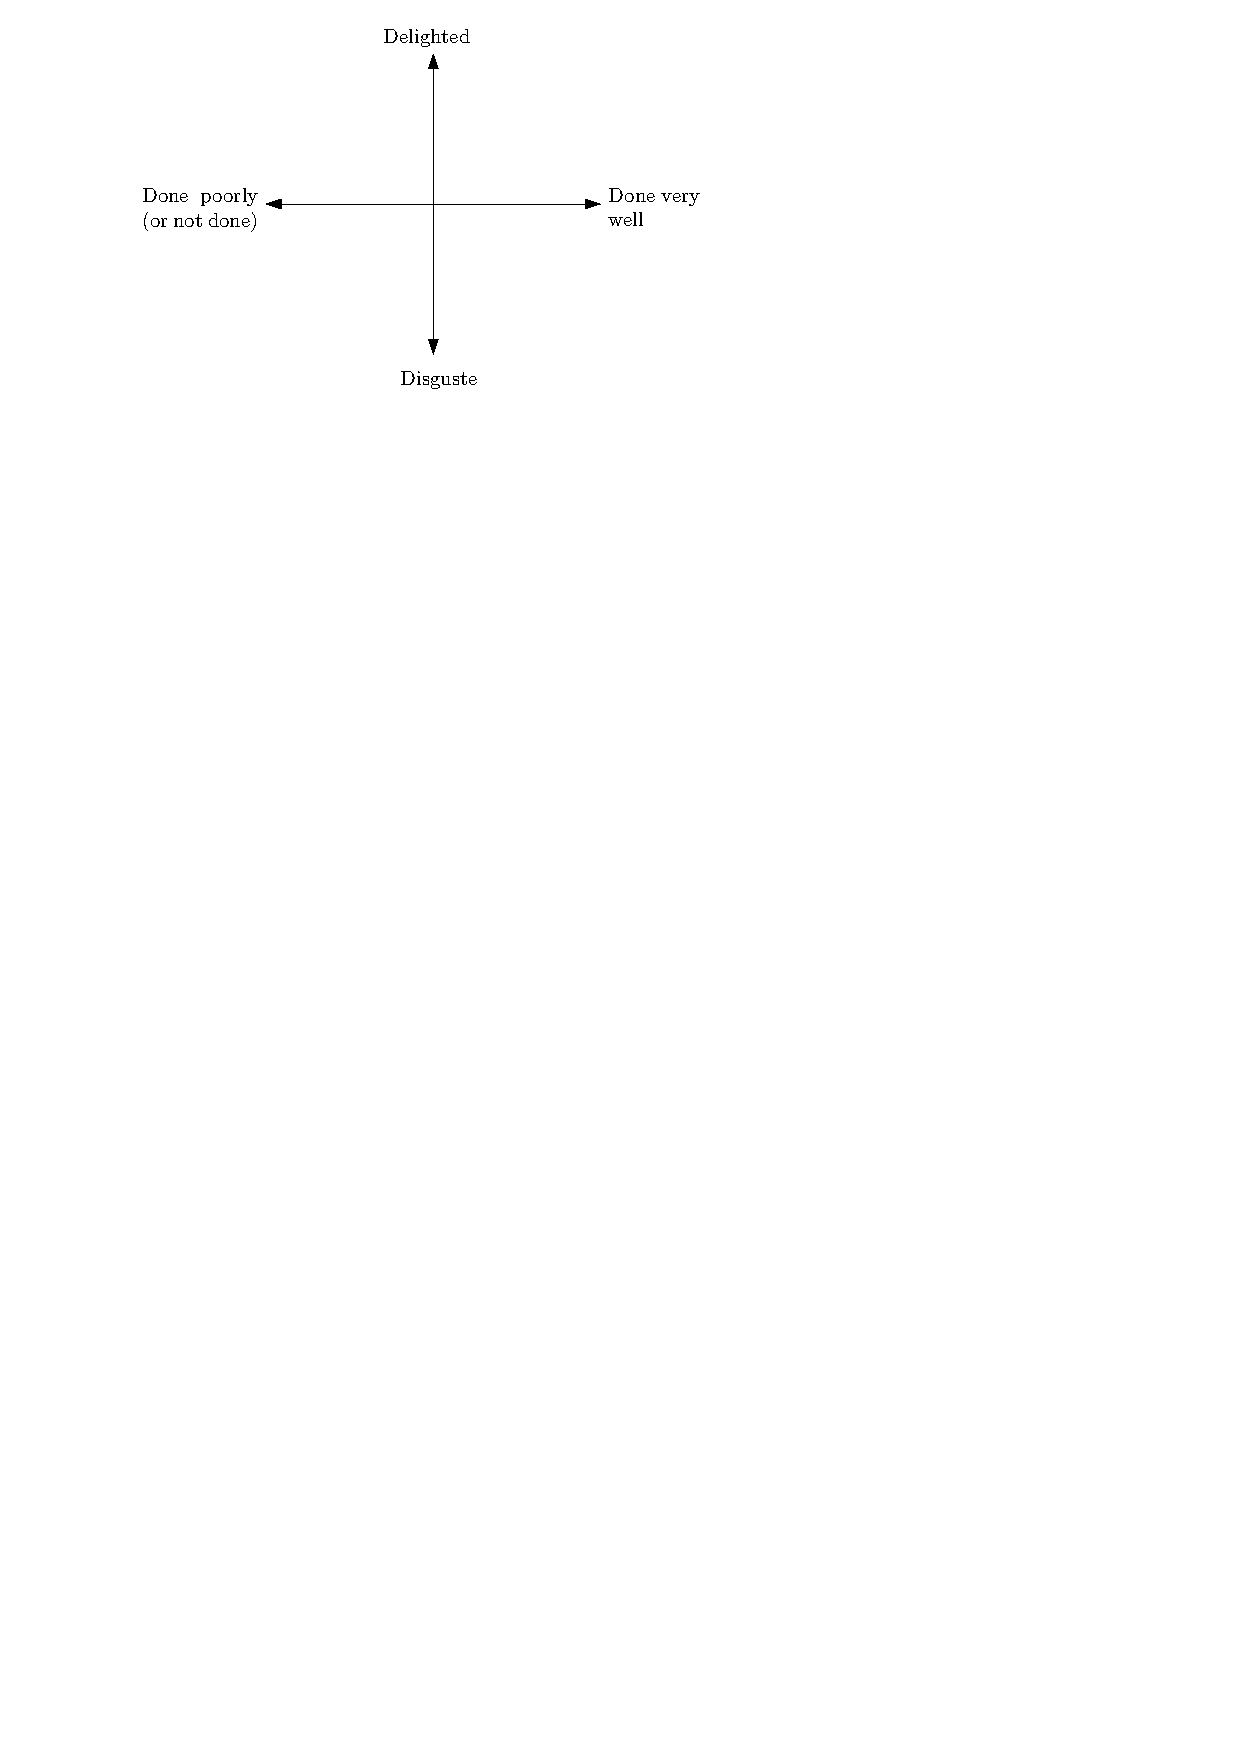
\includegraphics[width=0.3\textwidth]{\figs/kano}
    \caption{Modelo Kano}
\end{wrapfigure}
El modelo Kano es una herramienta analítica utilizada para relacionar las características de un producto con el nivel de satisfacción que estas derivaron al cliente final. Dicho modelo fue desarrollado por el profesor Nokiari Kano en Japón. El modelo tiene como objetivo primigenio poder determinar con precisión los atributos valorados por los consumidores para mejorar la satisfacción y crear o mejorar productos que cumplan con esos atributos valiosos. \cite{kanomodel} \par
El modelo Kano propone analizar las experiencias de los clientes basado en un gráfico, en el eje-x tenemos que tan buena ejecución tiene el producto o servicio y en el eje-y tenemos qué tan satisfecho está el cliente o que tan asqueado. \cite{videokano}

\section*{Cinco categorías del modelo Kano}
\begin{wrapfigure}{R}{0.3\textwidth}
    \centering
    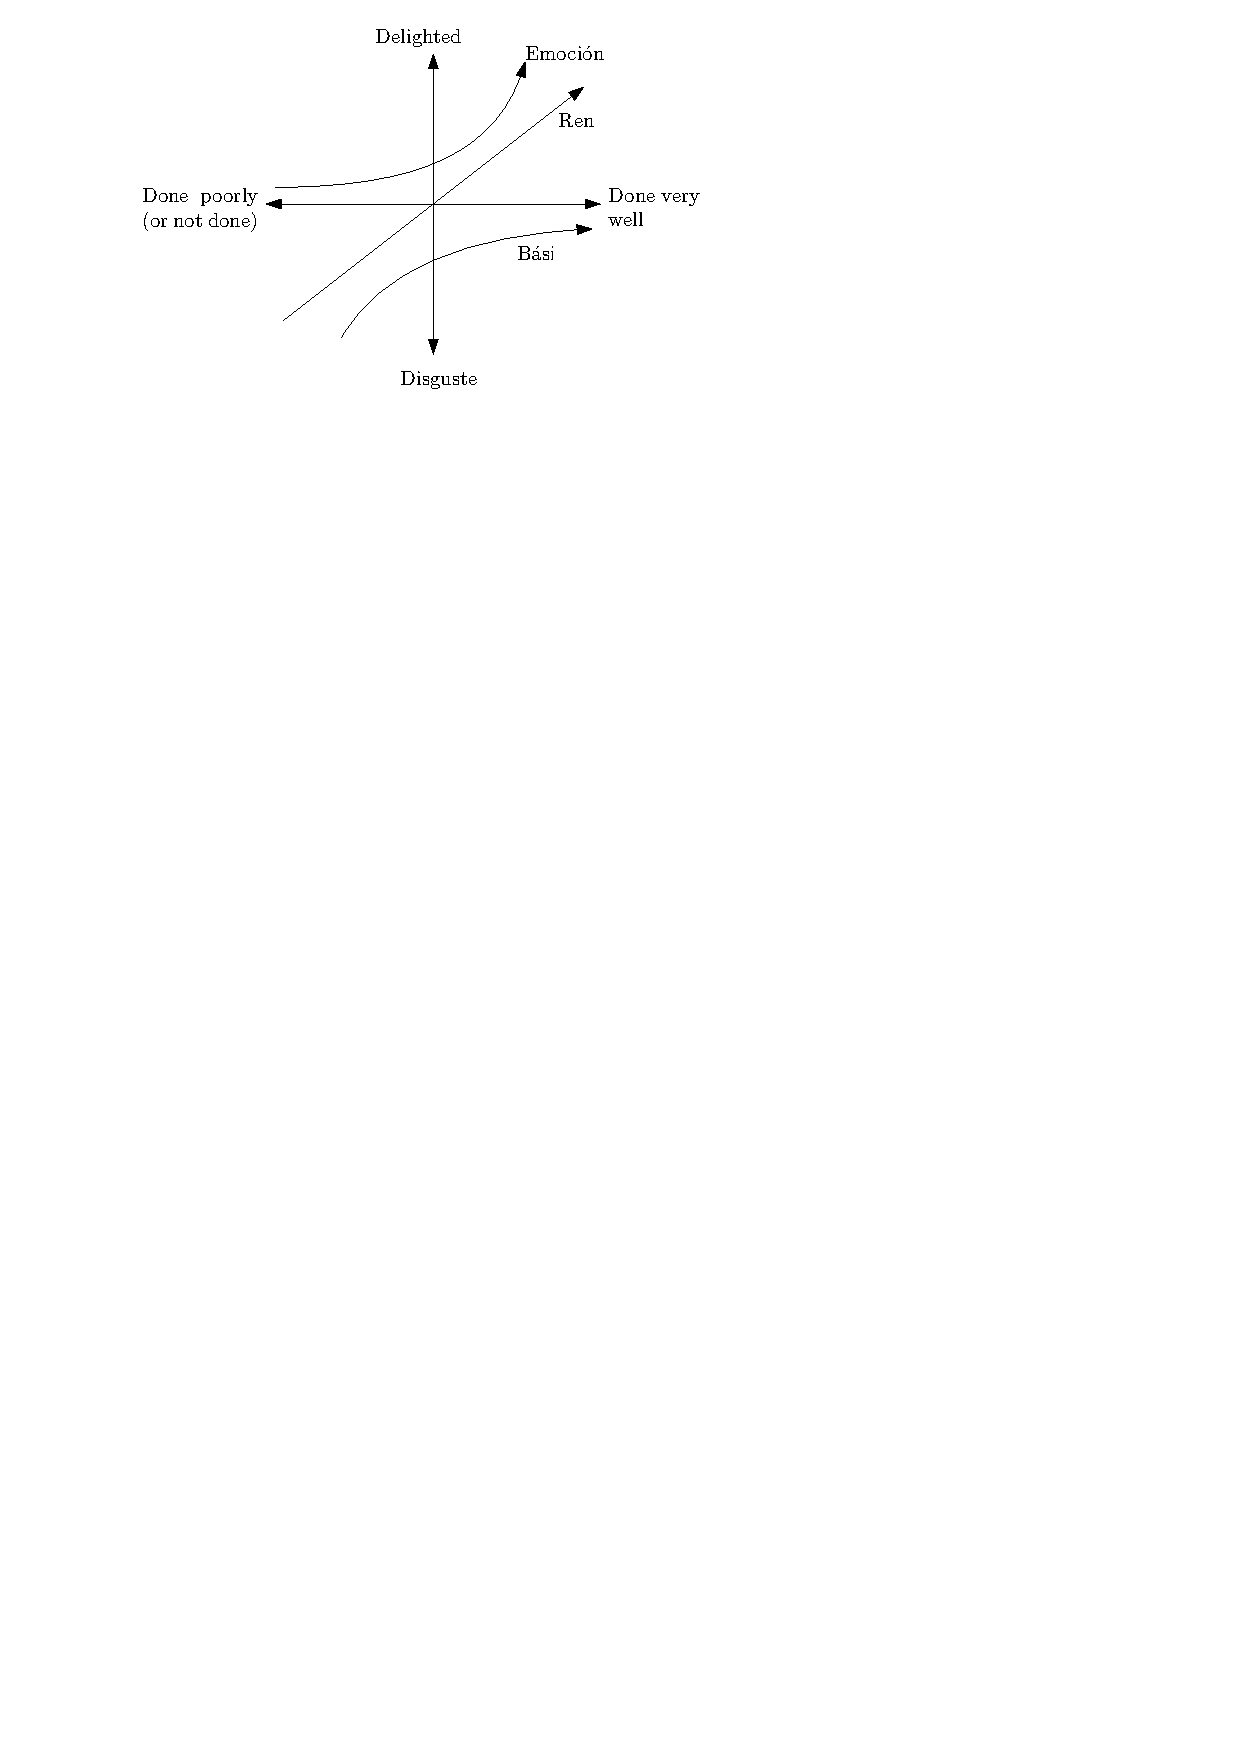
\includegraphics[width=0.3\textwidth]{\figs/kano1} 
\end{wrapfigure}
1. Calidad básica / esperada: Si se cumplen las personas van a estar neutrales por que es lo que esperaban del servicio. Si un usuario toma un vuelo y en su destino están las maletas a tiempo y bien, es lo que el usuario espera. \par
2. Calidad deseada / performance: estas son las cosas en las cuales se compiten, por ejemplo precio, comodidad, calidad. La regla es ``\emph{Más es mejor}''. Típicamente los usuarios se dan cuenta y comparan con la competencia. \par
3. Calidad motivadora / emocionante: el cliente no se lo espera y es neutral a estas necesidades, son por ejemplo, estoy viajando y una aerolínea me deja viajar en primera clase cuando yo pagué por el vuelo económico. Es una buena estrategia para diferenciación competitiva. Hay un elemento sorpresivo. Producen gran satisfacción al cliente pero su ausencia no generará insatisfacción.  \par
4. Calidad indiferente: atributos que sean como sean le dan absolutamente igual al cliente, por ejemplo, font de las letras, color de un teclado. \par
5. Calidad de rechazo: atributos que indican que el producto está defectuoso, por ejemplo, cubiertos plásticos que se rompen fácilmente. \par



\section*{Variantes a las categorías}
Al pasar el tiempo o al avanzar la tecnología lo que anteriormente se consideraba un lujo puede hoy considerarse una necesidad básica. Las preferencias de los consumidores también pueden ser muy variadas. 

\bibliographystyle{plain}
\bibliography{links.bib} 


%%%%%%%%%%%%%%%%%%%%%%%%%%%%%%%%%%%%%%%%%%%%%%%%%%%%%%%%%%%%%%%%%%%%%%%%%%%%%%%%%%%%%%%%%%%%%%%%%%%%%%%%%%%%%%%%%%%%%%%%%%%%%%%%%%%%%%%%%%%%%%
\end{document}

